\chapter{RC 3}
\recitation{3}{20 Oct. 18:30}{}

\section{Review}
Independence of random variables: 
\begin{exercise}
   Let \(X\) and \(Y\) be independent discrete random variables and let \(g, h:\mathbb{R} \to \mathbb{R}\). Show that \(g(X)\) and and \(h(Y)\) are independent. 
\end{exercise}

\subsection{Expectation}
\begin{theorem*}
   (Proposition 6. in \cite{Und_Chatterjee}). Let \(X_1,\dots , X_n\) be discrete random variables and 
   \(Y =f(X_1,\dots, X_n) \) for some function \(f\). Then,
   \[
    E(Y) = \sum_{x_1,\dots,x_n}f(x_1,\dots,x_n) P(X_1 = x_1, \dots, X_n = x_n).
   \] 
\end{theorem*}
With this notion we can use the linearity of expectation.
% From Bernoulli to Binomial 

\section{Applications}
\subsection{Geometric r.v}
\begin{eg}[Coupon collector problem]
    (\cite{Gravner2021} Example 8.6)
Sample from n cards, with replacement,
    indefinitely. Let N be the number of cards you need to sample for a complete collection, i.e., to
    get all different cards represented. What is \(E[N]\) ?
\end{eg}
\subsection{Piosson Approximation to binomial}

\begin{eg}[HW5,Q4]
(\cite{IntroPanchenko} Exercise 1.3.6)
When you bet on black in Roulette, your
chances are 18/38. Suppose also that bets over \$250 are not

allowed by the casino. You decide to play the following strat-
egy: you start with a \$1 bet and double the bet until either you

win (the same amount as the bet) or the bet exceeds \$250;
then you start again with a \$1 bet and repeat. We will call
this sequence of bets in the strategy until restart with a \$1
bet ‘one round’. If you play 1000 rounds of this strategy,
what is the probability that your total winnings/losses are
0? Compute the exact formula and then compare it with
Poisson approximation. 
\end{eg}
\textbf{Solution. } Suppose in the $i$-th round, $1\leq i\leq 1000$, the money you'll get if end up winning at the $n$-th bet is
\begin{equation*}
-1-2-\cdots-2^{n-2}+2^{n-1}=2^{n-1}-(2^{n-1}-1)=1,
\end{equation*}
which is independent to $n$. Otherwise, if you end up lose all the bets, then the money you'll earn is
\begin{equation*}
-1-2\cdots-2^7=-(2^8-1).
\end{equation*}
Note that the maximum number of bets is $8$ times since $2^8>250$. Clearly, you'll earn this amount with probability $q=(1-p)^8$. Therefore, $\mathbb{P}(\text{ends up getting $1$ dollar in a round})=1-q.$

Now define
\begin{equation*}
\begin{aligned}
&N=\text{total earning in $1000$ rounds} \\& 
W =\text{total number of rounds that ends up getting $1$ dollar} \\&
L =\text{total number of rounds that ends up getting $-255$ dollars}
\end{aligned}
\end{equation*}
Clearly $W+L=1000$, and
\begin{equation*}
N = 1\cdot W+(-255)\cdot L.
\end{equation*}
Moreover, one can see
\begin{equation*}
\mathbb{P}(L=k)=\binom{1000}{k}q^k(1-q)^{1000-k},
\end{equation*}
which is a $Bin(1000,q)$ random variable. Then
\begin{equation*}
\mathbb{P}(N\geq 0)=\mathbb{P}(W-255L\geq 0)=\mathbb{P}(1000-256L\geq 0)=\mathbb{P}(L<4).
\end{equation*}
Using Poisson approximation to $L$, one can get
\begin{equation*}
\big|\mathbb{P}(L<4)-\mathbb{P}(X<4)\big|\leq\frac{\lambda^2}{1000},
\end{equation*}
if $\lambda = 1000q$ and $X\sim Pois(\lambda)$.


\section{Variance}
Variance of a random variable \(X\) is the second moment of the demeaned \(X-E[X]\), i.e
\[
    \text{Var} (X) = E[(X-E[X])^2] = E[X^2] - E[X]^2
\]
\begin{eg}
    Calculate the variance of Poisson random variable
\end{eg}
\textbf{Note}: Second moments for some random variable may not exists (\(L^2\) will be save ), and in those cases, the variance will not be defined. See Cauchy distribution.
\section{Covariance}
\begin{figure}[h]
    \centering
    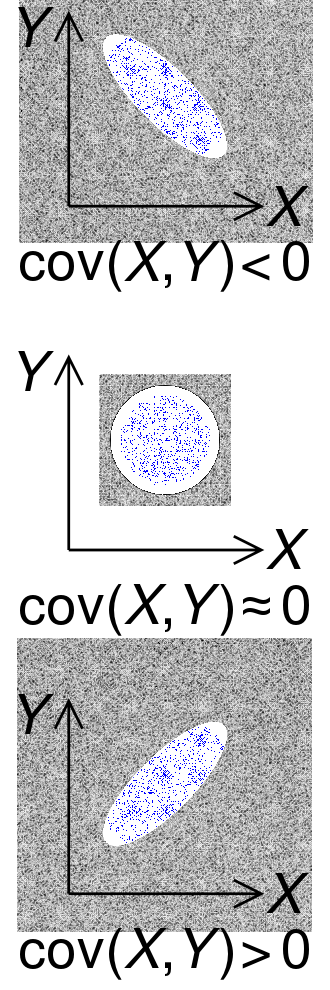
\includegraphics[width=0.3\textwidth]{./Figures/Covariance_trends.png}
    \caption{From wiki}
\end{figure}


\section{Extra note}
%\subsection{Estimate the error bound}


% The error bound Theorem 1.1
% Example of Poisson
% Panchenko Lemma 1.2 as practice of adv. cal. (Why do we need to have integrable)
% Or stability of Poisson